\documentclass[aspectratio=169]{beamer}
\usetheme{Berlin}
\usecolortheme{beaver}


\usepackage[utf8]{inputenc}
%\usepackage[T1]{fontenc}
%\usepackage{lmodern}
\usepackage{amsmath,amssymb,amsthm,mathrsfs,amsfonts, amstext}  
\usepackage{mathtools}
\usepackage{listings}
\usepackage[english]{babel}
\usepackage{verbatim}
\usepackage{pgfplots}
%\usepackage{amssymb, amsmath, amsbsy} % simbolitos
%\usepackage{upgreek} % para poner letras griegas sin cursiva
%\usepackage{cancel} % para tachar
%\usepackage{mathdots} % para el comando \iddots
%\usepackage{mathrsfs} % para formato de letra
%\usepackage{stackrel} % para el comando \stackbin
\usepackage{graphicx}
\usepackage{grffile}
\graphicspath{ {../images/} }
\usepackage{caption}
\usepackage{chngcntr}
\usepackage{etoolbox} % needed for the code below
\usepackage{hyperref}
\usepackage{multimedia}
\usepackage{algpseudocode}
\usepackage{tikz}
\usepackage{IEEEtrantools}
\usepackage{physics}
\usepackage{pgfpages}
\usepackage{booktabs}
\usepackage{amsfonts}
\usepackage{siunitx}
%\setbeameroption{show only notes}
%\setbeameroption{show notes on second screen=right}
\DeclareMathOperator{\Ra}{Ra}
\newcommand{\jump}[1]{\ensuremath{[\![ #1 ]\!]}}
\newcommand{\avg}[1]{\ensuremath{\{\mspace{-6mu}\{#1\}\mspace{-6mu}\}}}

\let\oldfootnotesize\footnotesize
\renewcommand*{\footnotesize}{\oldfootnotesize\tiny}

\AtBeginSection[]
{
	\begin{frame}
	\frametitle{Overview}
	\tableofcontents[currentsection]
	\end{frame}
}

\setbeamercolor{block title}{use=structure,fg=white,bg=red!75!black}
\setbeamercolor{block body}{use=structure,fg=black,bg=red!5!white}
\setbeamertemplate{itemize item}{\color{red!90!black}$\blacktriangleright$}
\setbeamertemplate{itemize subitem}{\color{red!50!black}$\blacktriangleright$}
\setbeamercolor{section number projected}{fg=white,bg=red!60!black}
\setbeamercolor{subsection number projected}{parent=section number projected}


\bibliographystyle{alpha}


%%%%%%% math definitions %%%%%%%%%%


%%%%%%%%%%%%%%%%%%%%%%%%%%%%%%%%%%%%%%%%%%%%%%


%%%%%%%%%%%%%%%%%%%%%%%%%%%%%%%%%%%

\title{Deep Potential Molecular Dynamics: a scalable model with the accuracy of quantum mechanics - A summary \cite{PhysRevLett.120.143001}}
\author{Jonas Wildberger}
\begin{document}

\begin{frame}
  \titlepage
\end{frame}

\begin{frame}{Overview}
  \tableofcontents
\end{frame}

\section{Motivation}
\begin{frame}{Motivation}

		\begin{itemize}
			\item Trade-off: Accuracy vs. Efficiency
			\begin{center}
			\begin{tabular}{SS} \toprule
				{AIMD} & {EFF} \\ \midrule
				\text{small space- and timescales}  & \text{larger scales} \\
				\text{high accuracy}  & \text{approximative in nature}  \\ \midrule
			\end{tabular}
		\end{center}
			\item ML so far: Auxiliary quantities to preserve symmetries\\
			 $\Rightarrow$ Assign local reference frames to each atom and leverage extensive character of potential energy
			 $$E = \sum_i E_i$$
			
		\end{itemize}
\note{AIMD: First principles, quantum mechanics, DFT. Computational costs: 100 ps, 100s of atoms, empirica FF: based on approximations and experimental data}
\note{Data: Atomic configurations and corresponding potential energies, learn this functional dependence}
\note{real system invariant to permutations, translations, rotations, so model needs too. Auxiliary quantities: Symmetry functions (describe local geometric environment, problem: ad hoc), coulomb matrix entries: distinct inverse distances between all atoms, problem: extened periodic systems}
\end{frame}
\note{Convection: transfer of heat by the movement of the fluid\\
	Natural: motion generated by density differences, not by external sources\\
Applications: Nuclear reactor design,
cooling of electronic eqiupment,
heating and ventialtion in the design
of buildings\\
Goal: Identify different flow patterns and investigate which method is suited better}

\section{The model}
\begin{frame}{First step}
	\begin{columns}
		\begin{column}{0.5\textwidth}
			\begin{itemize}
				\item<1-> Local coordinate frame for each atom with atom at center
				\item<2-> $\mathbf D_i = (\mathbf D_{ij})_j$ input for NN, where $j$ covers all neighbors within cutoff radius $R_c$, sorted by chemical species, inverse distances
				\item<3-> Theoretical foundation: Embedded Atom Concept
			\end{itemize}
		\end{column}
		\begin{column}{0.5\textwidth}
			\begin{figure}
				
				\centering
				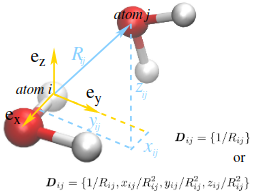
\includegraphics[width=0.8\textwidth]{MD}
				\caption{Geometry of the local coordinate frames \cite{PhysRevLett.120.143001}}
			\end{figure}
		\end{column}
	\end{columns}
\note{Embedded Atom Concept: Energy sum of functions of seperation of atom and neighbors. Reciprocal distances: Reduce weight of distant neighbors}
\note{Figure: Water, e x O-H bond, e z perpendicular to plane of water molecule }
\note{other option for D i j angular information as well x ij cartesian coordinates of R i j}
\end{frame}
\begin{frame}{Second step}
\begin{columns}
	\begin{column}{0.5\textwidth}
\begin{itemize}
	\item<1-> Fully connected NN consisting of 5 hidden layers with 240, 120, 60, 30, 10 units resp.
	\item<2-> $\tanh $ activation for hidden layers and identity for output
	\item<3-> Adam optimizer 
\end{itemize}
\end{column}
\begin{column}{0.5\textwidth}
	\begin{figure}
		
		\centering
		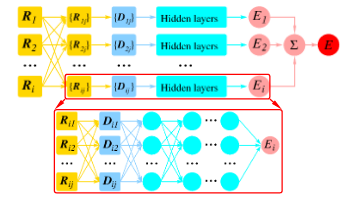
\includegraphics[width=0.8\textwidth]{MD1}
		\caption{Visualisation of the NN \cite{PhysRevLett.120.143001}}
	\end{figure}
\end{column}
\end{columns}
\note{NN: fixed input size, append 0s potentially}
\end{frame}
\begin{frame}{Loss function}
$$\mathcal L (p_\epsilon, p_f, p_\xi) = p_\epsilon \Delta \epsilon^2 + \frac{p_f}{3N} \sum_i |\Delta \vec F_i|^2 + \frac{p_\xi}{9} \norm{\Delta \Xi}^2$$
$\Delta:$ Difference between prediction and training data, $N:$ number of atoms, $\epsilon:$ energy per atom, $\vec F_i:$ Force on atom $i$, $\Xi:$ Virial tensor $\Xi = -\frac{1}{2} \sum_i \vec R_i \otimes \vec F_i$
\vspace{.3cm}
\begin{itemize}
	\item<2-> Key difference: Inclusion of forces and virial tensor for regularisation
	\item<3-> Parameters $p_\epsilon, p_\xi$ steadily increased during training, $p_f$ steadily decreased
\end{itemize}
\note{Virial: comparison of kinetic, potential energy}
\end{frame}
\section{Summary}
\begin{frame}{Summary}
\visible<1->{Advantages:}
\begin{itemize}
	\item<2-> High accuracy: Similar performance to AIMD simulations for water, slightly better than GDML benchmark for molecules
	\item<3-> Scalable and parallelisable: Computational costs increase only linearly with the number of atoms
	\item<4-> Simplicity: No auxiliary quantities as opposed to other ML methods 
\end{itemize}
\visible<5->{Disadvantages:}
\begin{itemize}
	\item<6-> Discontinuities in results due to sharp cutoff radius
	\item<7-> Long-range coulomb interactions neglected, see \cite{article}
\end{itemize}
\note{GDML: gradient domain machine learning}
\note{not chemically accurate, since still approximative, but way better than empirical FFs}
\note{Coulomb: electrostatic forces over distances outside curoff radius}
\end{frame}

\begin{frame}{References}
\bibliography{literatur}
\end{frame}
\end{document}